\documentclass{exam}

\usepackage{graphicx}
\usepackage{amssymb}
\usepackage[T1]{fontenc}
% \usepackage{wrapfig}

\graphicspath{ {../res/} }

\title{Triathlon - Maths}
\author{Olympiad Maths}
\date{May 2022}

\pagestyle{plain}
\marksnotpoints

\begin{document}
\large
\maketitle

\begin{center}
    \vspace{-10pt}
    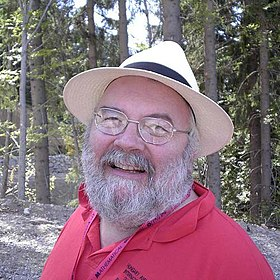
\includegraphics[height=100pt]{geoffsmith}
    \vspace{-10pt}
\end{center}

\section* {Instructions}

Read these before attempting the questions.

\subsection*{Time: 4 hours}

\subsection*{Format}
This paper has 6 available questions each worth 10 marks.\\
Make sure to write full written proofs where possible.

\subsection*{Tools}
Rulers and compasses are allowed, but no protractors or calculators.

\subsection*{Submission}
Submit your paper by dm to
{\fontfamily{cmss}\selectfont e=pi=3\#5257}
before \textbf{23:59 on Sunday 22nd May}.\\
Please scan in then send as a \textbf{single PDF}. Online tools are available for this.\\
On the front page, write your \textbf{discord ID} (right click username -> copy ID).\\
After submission, you can be added to a channel to discuss the questions. Please don't discuss them outside of that channel.

\centering

\vspace{\stretch{1}}
\textbf{The questions begin on the next page.}\\
\vspace{10pt}
Good luck, and most importantly have fun!
\vspace{\stretch{1}}



\newpage
\section*{Questions}
\vspace{20pt}

\begin{questions}
    \question
    Two numbers $a$ and $b$ satisfy the equations $a+b=2$ and $a^2+b^2=6$.
    \begin{parts}
        \part What is the value of $a^3+b^3$?
        \part What is the value of $a^6+b^6$?
    \end{parts}
    \vspace{\stretch{1}}

    \question
    In triangle $ABC$, $M$ is the midpoint of $BC$. Let $P$ be a point on $AM$, inside triangle $ABC$.
    Rays $BP$ and $CP$ meet segments $AC$ and $AB$ at $D$ and $E$ respectively. Let the circles with diameters $BD$ and $CD$ meet at $X$ and $Y$.

    Show that $A, X, Y$ are collinear.
    \vspace{\stretch{1}}

    \question
    There are $n$ sweets in a pile. Alice and Bob take turns eating the sweets (Alice starts). Each turn, they eat either one sweet, or a prime number of sweets that divides the current number of sweets in the pile.

    For what values of $n$ can Bob eat the last sweet?
    \vspace{\stretch{1}}

    \question
    Find all functions $f : \mathbb{R} \to \mathbb{R}$ such that for all $x, y \in \mathbb{R}$:
    $$f(x^2+y) = f(f(x)-y) + 4f(x)y$$

    \question
    The six members of the illuminati have designed a world-ending robot. They wish to give it ample safeguarding though, so they lock up the robot inside an indestructible case, using multiple locks that each have different fitting keys. The group wishes to distribute lock keys among themselves so that the robot can be released when and only when three or more members are present. What is the minimum possible number of locks needed? What is the minimum possible number of keys each member must carry?
    \vspace{\stretch{1}}

    \question
    Define the sequences $x_n, y_n$ as follows:
    \begin{itemize}
        \item
        $x_0 = 1, y_0 = 2$
        \item
        $x_{n+1} = \frac{x_n + y_n}{2}$
        \item
        $y_{n+1} = \sqrt{x_{n+1}y_n}$
    \end{itemize}

    Show that $\lim_{n \to \infty} y_n$ exists, and find its value.

\end{questions}


\vspace{\stretch{1}}
\centering \LARGE \textbf{END OF PAPER}
\vspace{\stretch{1}}
\end{document}
